\documentclass[10pt]{article}

\usepackage{tabularx}
\usepackage[a4paper,margin=2.5cm, bottom=2.5cm]{geometry}
\usepackage{fancyhdr}
\usepackage{listings}
\usepackage{booktabs}
\usepackage{float}
\usepackage{subcaption}
% \usepackage{caption}
% \captionsetup{font=footnotesize}
\usepackage{graphicx}
\usepackage{amsmath}
\usepackage{amssymb}
\usepackage{amsthm}
\usepackage{array}
\usepackage[table]{xcolor}
\usepackage{pgfplots}
\pgfplotsset{compat=1.17}
\usepackage{pgfplotstable}
\usepackage{multirow}
\usepackage{tikz}
\usepackage[hidelinks]{hyperref}
\usepackage{titling}
\usepackage[polish]{babel} % Polish language support

\setlength{\headheight}{40pt}
\setlength{\parindent}{0pt}
\setlength{\parskip}{1ex}
\renewcommand{\headrulewidth}{0pt}

\pagestyle{fancy}
\fancyhead{}
\fancyhead[L]{
    \renewcommand{\arraystretch}{1.5}
    \begin{tabularx}{\textwidth}{|X|X|}
        \hline
        \bfseries Obliczenia inteligentne & \bfseries \thetitle \\
        \hline
    \end{tabularx}
}
\fancyfoot[C]{\thepage}

\renewcommand{\maketitle}{
    \thispagestyle{plain}
    \renewcommand{\arraystretch}{2}
    \vspace*{-8em}
    \footnotesize
    \begin{flushleft}
        \begin{tabularx}{\textwidth}{|X|X|}
            \hline
            \bfseries Obliczenia Inteligentne  & \bfseries \thetitle                           \\ \hline
            \multicolumn{2}{|l|}{
                \begin{tabular}[t]{@{}ll@{}} 
                    \textbf{Grupa:} Grupa 1
                    \hspace{4.5em}
                    \textbf{Dzień i czas:} Czwartek, 10:00
                    \hspace{4.5em}
                    \textbf{Rok akademicki:} 2023/24
                \end{tabular}
            } \\ \hline
            \multicolumn{2}{|l|}{
                \begin{tabular}[t]{@{}l@{\hspace{10em}}l@{}} 
                    \textbf{Imię i nazwisko:} \textsc{Jakub Pawlak} & \textbf{Imię i nazwisko:} \textsc{Magdalena Paku\l a} 
                \end{tabular}
            } \\
            \hline
        \end{tabularx}
    \end{flushleft}
    \renewcommand{\arraystretch}{1}
}


\title{Projekt 2 --- Zadanie 1}
\captionsetup{font=small}
\begin{document}
\maketitle
\normalsize
\section{Opis ekstrakcji cech --- Osoba 1 (Magdalena Pakuła)}

\paragraph*{Principal Component Analysis (PCA)} - Analiza głównych składowych technika redukcji wymiarowości, która pomaga w przekształcaniu danych wielowymiarowych w postać niskowymiarową, przy jednoczesnym zachowaniu jak największej oryginalnej zmienności.
Metoda PCA standaryzuje dane, oblicza macierz kowariancji rejestrującą relacje między cechami, a następnie dekomponuje ją na wartości własne i wektory własne. Wektory własne reprezentują kierunki największej wariancji, a wartości własne jej wielkość. Po posortowaniu wartości własnych malejąco, wybierane są największe z nich i odpowiadające im wektory własne do utworzenia nowej przestrzeni cech. Dane są rzutowane na tę przestrzeń, co skutkuje zbiorem danych o zredukowanej liczbie wymiarów, zachowującym najważniejsze informacje.
W kontekście danych MNIST, PCA może być stosowana do redukcji liczby wymiarów obrazów cyfr, co ułatwia ich analizę i wizualizację, a także przyspiesza trening modeli uczenia maszynowego poprzez zmniejszenie ilości przetwarzanych danych przy jednoczesnym zachowaniu istotnych informacji.

\begin{figure}[H]\centering
    \begin{subfigure}{0.16\textwidth}
        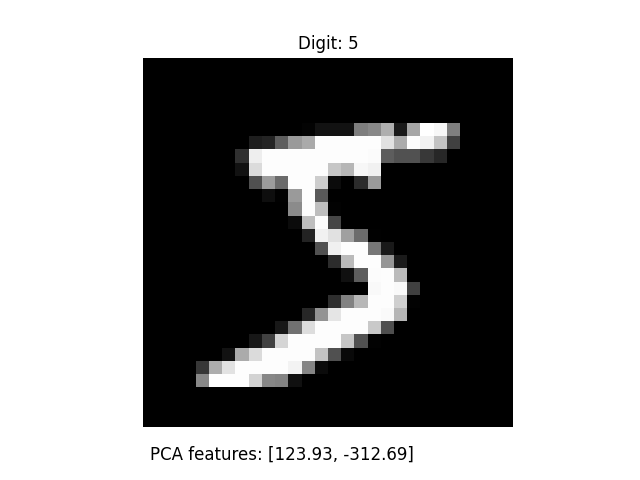
\includegraphics[width=\linewidth]{img/PCA/PCA_5}
        \caption{Wektor 2 cech dla liczby "5"}
    \end{subfigure}
    \hfill
    \begin{subfigure}{0.16\textwidth}
        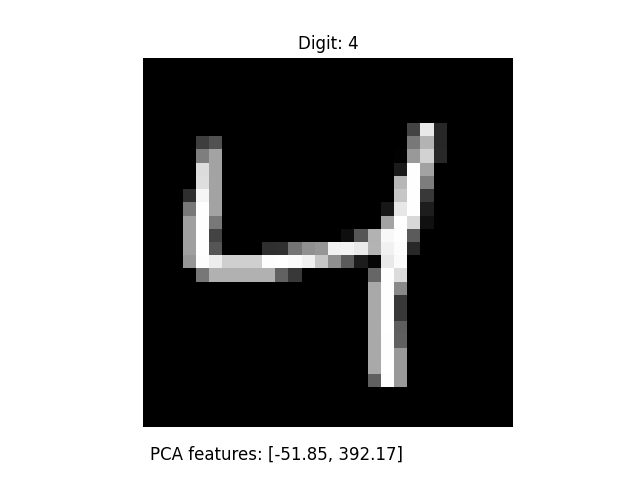
\includegraphics[width=\linewidth]{img/PCA/PCA_4}
        \caption{Wektor 2 cech dla liczby "4"}
    \end{subfigure}
    \hfill
    \begin{subfigure}{0.16\textwidth}
        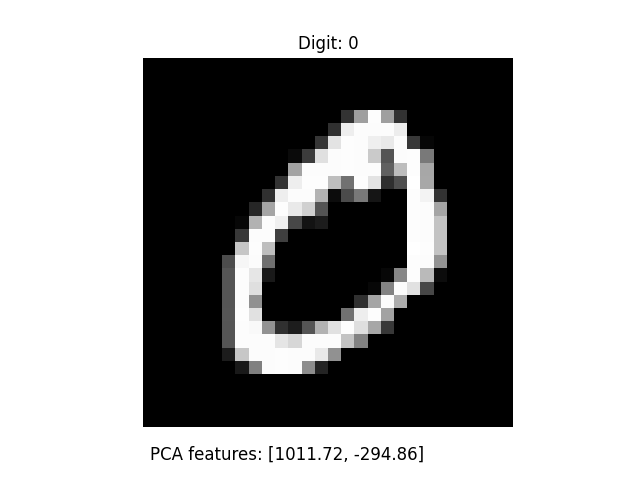
\includegraphics[width=\linewidth]{img/PCA/PCA_0}
        \caption{Wektor 2 cech dla liczby "0"}
    \end{subfigure}
    \hfill
    \begin{subfigure}{0.24\textwidth}
        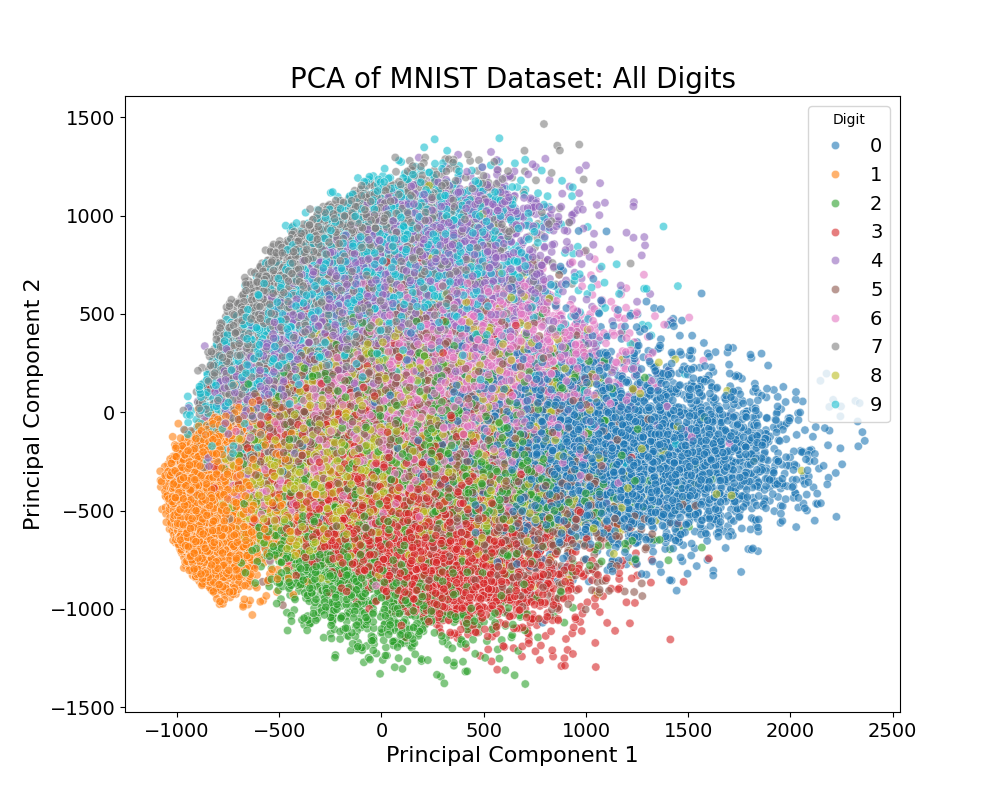
\includegraphics[width=\linewidth]{img/PCA/PCA_distribution}
        \caption{Rozkład cech PCA dla zbioru danych MNIST dwóch głównych składowych}
    \end{subfigure}
    \hfill
    \begin{subfigure}{0.24\textwidth}
        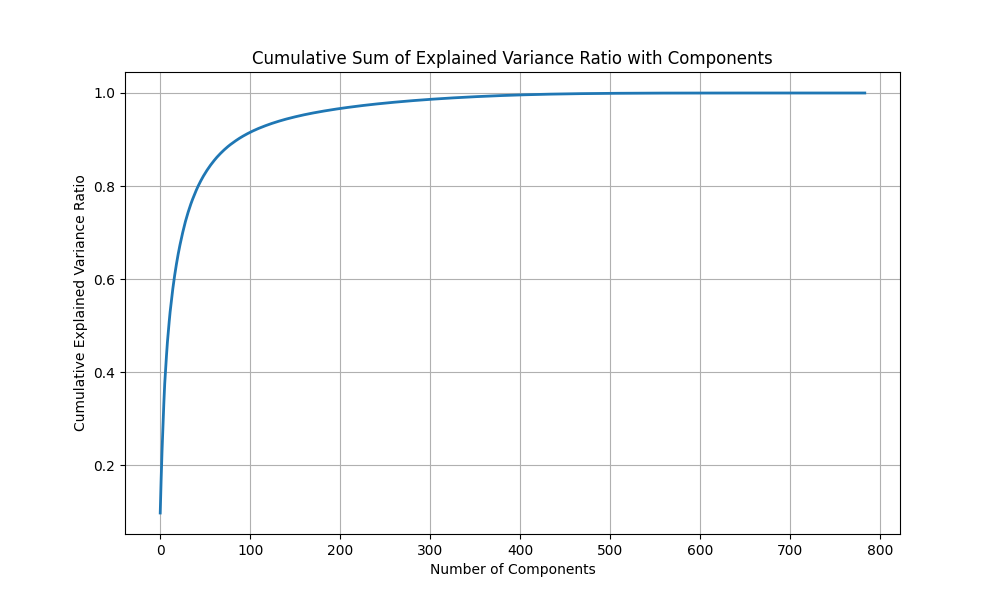
\includegraphics[width=\linewidth]{img/PCA/PCA_cumulative_variance}
        \caption{Skumulowana suma wyjaśnionej wariancji w funkcji liczby składowych}
    \end{subfigure}
    \caption{Przykłady ekstrakcji cech metodą PCA}
\end{figure}

%Na poniższym wykresie (rys.2) można zauważyć,jak poszczególne klasy cyfr (oznaczone różnymi kolorami) są rozmieszczone w przestrzeni dwuwymiarowej.
%Na wykresie obok (rys.3) pokazano skumulowaną sumę wyjaśnionej wariancji w funkcji liczby głównych składowych. Wykres ten pomaga zrozumieć, ile składowych jest potrzebnych do zachowania określonego poziomu całkowitej wariancji w danych.


\paragraph*{Binary Patterns (LBP)} - Lokalne wzorce binarne to technika ekstrakcji cech używana głównie w analizie obrazów, która przekształca obraz w zestaw wartości binarnych opisujących teksturę.
Proces ten polega na porównywaniu każdego piksela z jego sąsiadami.
Piksel centralny jest traktowany jako próg, a każdy sąsiedni piksel jest porównywany do tego progu.
Jeśli wartość sąsiada jest większa lub równa wartości centralnego piksela, przypisywana jest wartość 1, w przeciwnym razie 0. Wynikowe wartości binarne są następnie łączone w jednolitą wartość, która reprezentuje wzorzec tekstury w danym obszarze obrazu.
Metoda LBP jest odporna na zmiany jasności i kontrastu, co czyni ją użyteczną w różnych zastosowaniach, takich jak rozpoznawanie twarzy czy klasyfikacja tekstur. W przypadku danych MNIST, LBP może być używane do ekstrakcji cech, które są następnie wykorzystywane do klasyfikacji obrazów cyfr.

\begin{figure}[H]\centering
    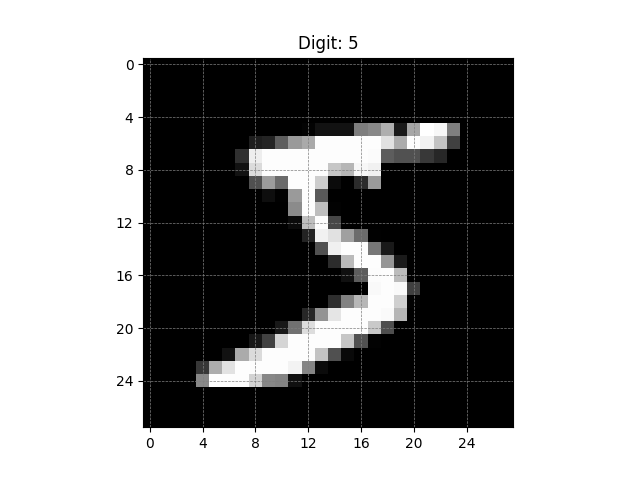
\includegraphics[width=.16\linewidth]{img/MNIST_5}
    \hfill
    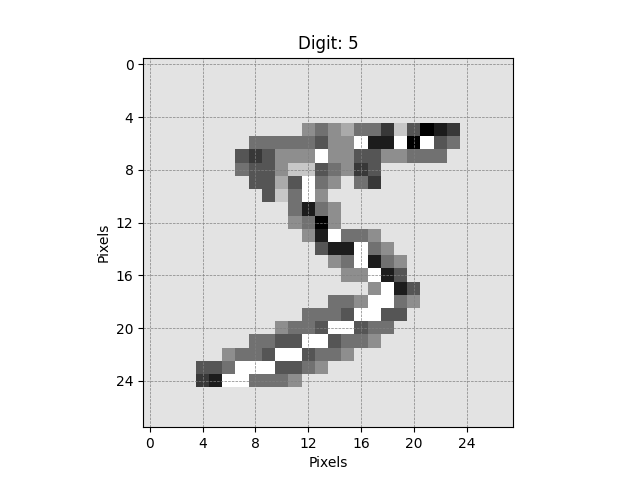
\includegraphics[width=.16\linewidth]{img/LBP/LBP_5}
    \hfill
    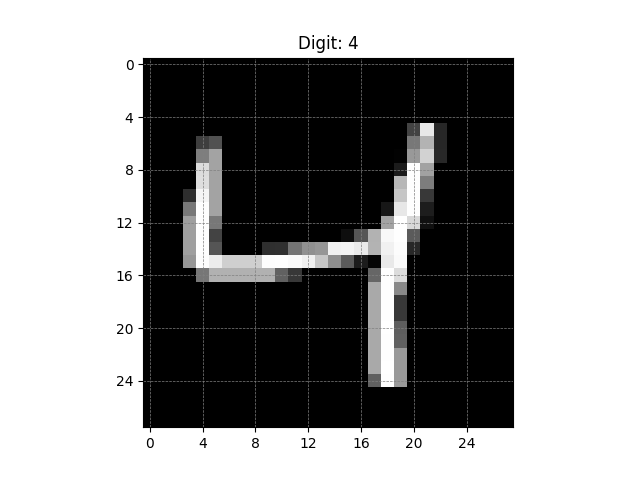
\includegraphics[width=.16\linewidth]{img/MNIST_4}
    \hfill
    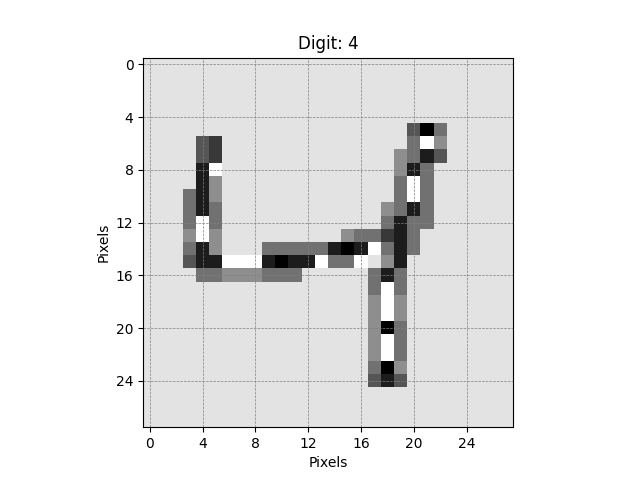
\includegraphics[width=.16\linewidth]{img/LBP/LBP_4}
    \hfill
    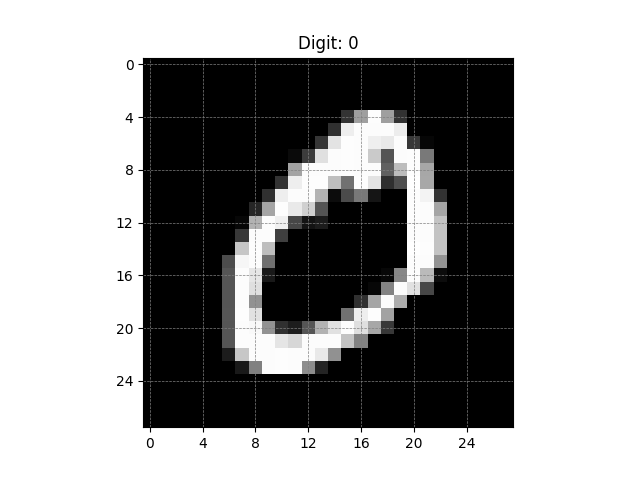
\includegraphics[width=.16\linewidth]{img/MNIST_0}
    \hfill
    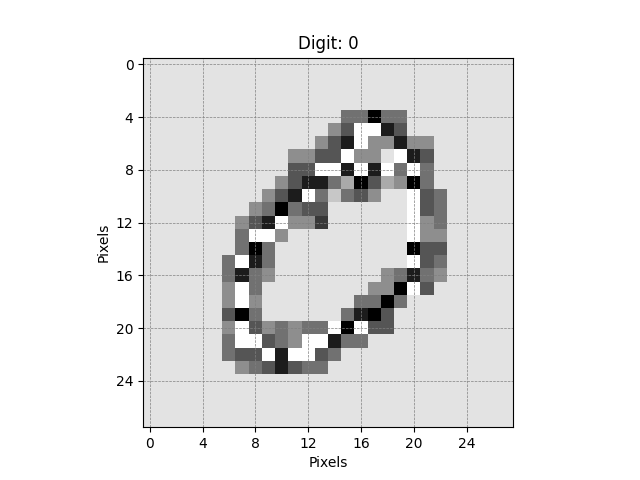
\includegraphics[width=.16\linewidth]{img/LBP/LBP_0}
    \caption{Przykłady ekstrakcji cech metodą LBP}
\end{figure}

\begin{figure}[H]\centering
    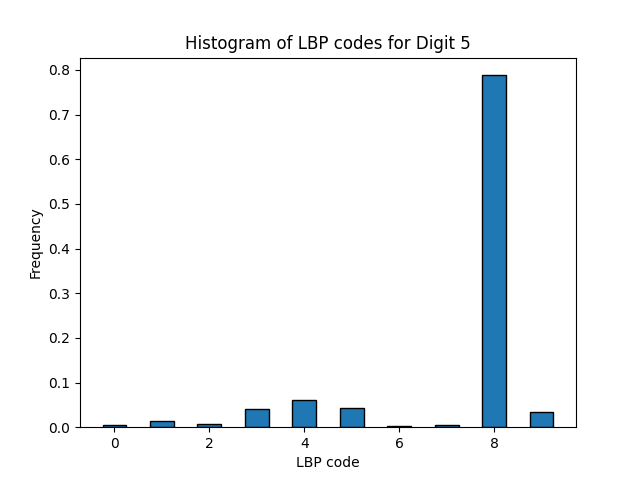
\includegraphics[width=.19\linewidth]{img/LBP/LBP_histogram_5}
    \hfill
    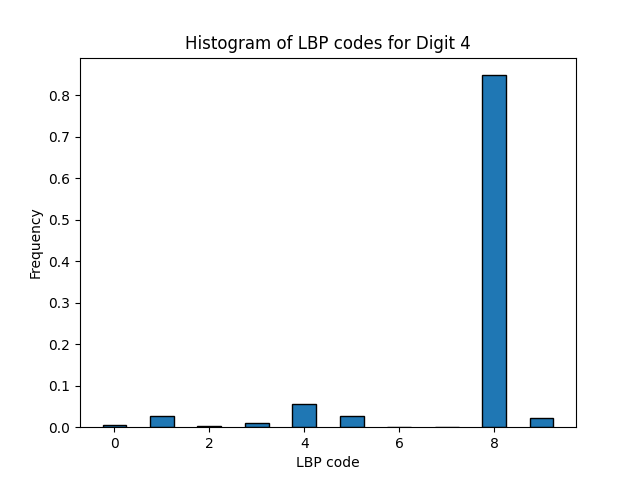
\includegraphics[width=.19\linewidth]{img/LBP/LBP_histogram_4}
    \hfill
    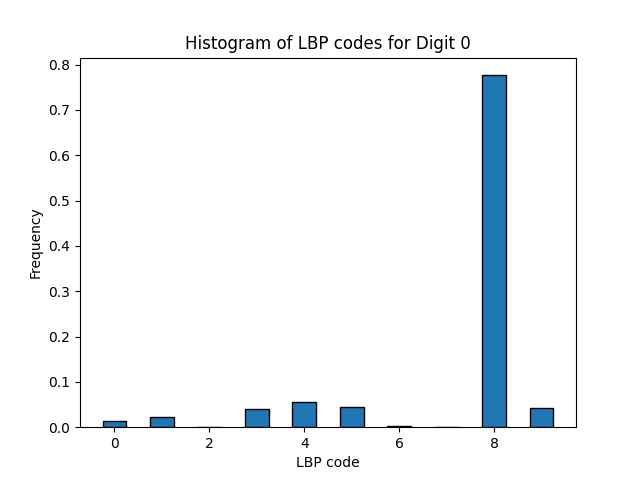
\includegraphics[width=.19\linewidth]{img/LBP/LBP_histogram_0}
    \caption{Histogramy LBP dla cyfry 0}
\end{figure}


\pagebreak

\section{Wyniki eksperymentu --- Osoba 1 (Magdalena Pakuła)}
\pagebreak

\section{Opis ekstrakcji cech --- Osoba 2 (Jakub Pawlak)}

\paragraph{Histogram of Oriented Gradients (HOG)} to metoda ekstrakcji cech używana w przetwarzaniu obrazu.
Opiera się ona na zliczaniu gradientów zorientowanych w tym samym kierunku, w określonych fragmentach obrazu.
Deskryptor HOG opisuje kształt obiektu na obrazie, więc bardzo dobrze nadaje się do zadania rozpoznawania cyfr, ponieważ następuje ono właśnie na podstawie kształtu.

Alorytm najpierw dzieli obraz na komórki o określonym rozmiarze. W przypadku zbioru MNIST użyto komórek $14\times14$, uzyskując podział całego obrazu na 4 komórki.
W każdej komórce, oblicza się dla każdego piksela lokalny gradient.
Następnie, wewnątrz każdej komórki zlicza się gradienty w określonych kierunkach i tworzy się z nich histogram.
Aby umożliwić wykrycie linii zarówno ortogonalnych jak i ukośnych, liczba kierunków została ustawiona na 9.
W celu poprawy jakości, wartości gradientów są dodatkowo normalizowane w większych grupach.
W tym przypadku, użyto grup o rozmiarze $2\times2$ komórek, co odpowiada całemu obrazowi.

Cały obraz zostaje zatem opisany za pomocą 4 komórek, każda zawierająca wartości dla 9 kierunków.
W ten sposób obraz $28\times28$ zredukowano do 36-elementowego wektora.

\begin{figure}[H]\centering
    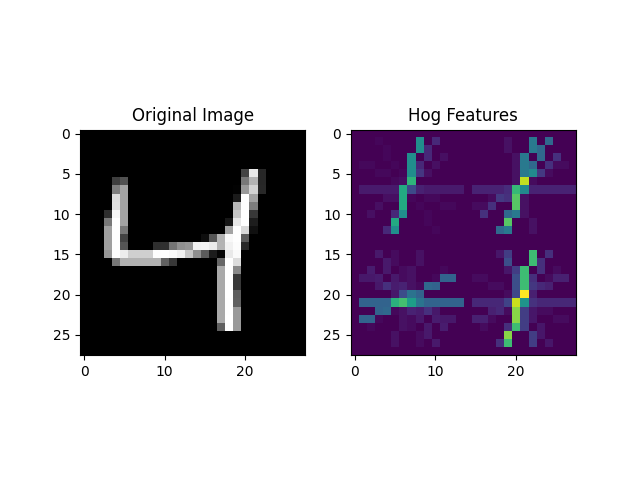
\includegraphics[width=.32\linewidth]{img/hog_vis/4.png}
    \hfill
    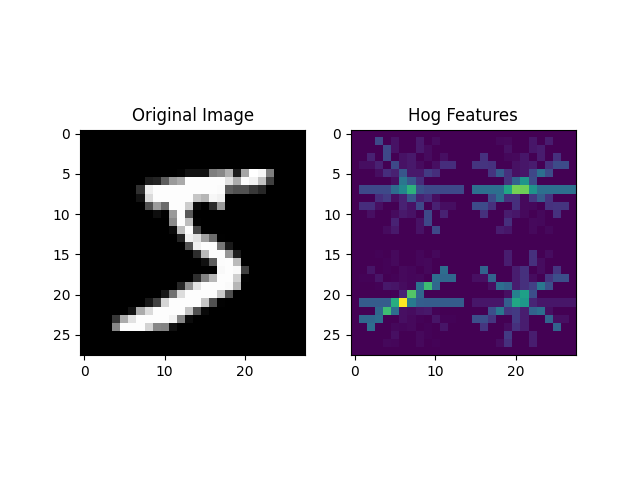
\includegraphics[width=.32\linewidth]{img/hog_vis/5.png}
    \hfill
    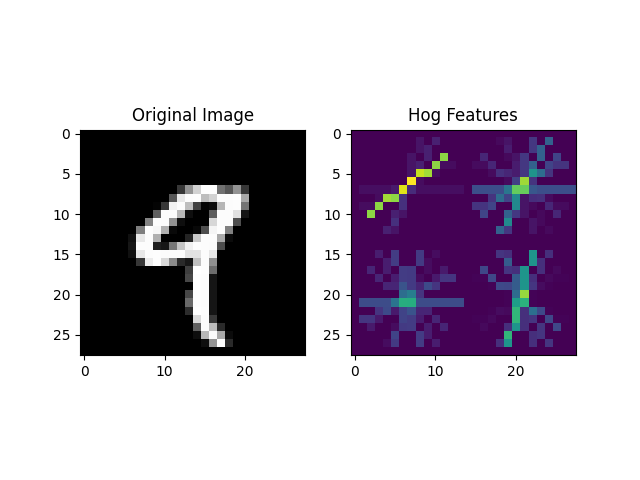
\includegraphics[width=.32\linewidth]{img/hog_vis/9.png}
    \caption{Przykłady ekstrakcji cech metodą HOG}
\end{figure}




\paragraph{t-Distributed Stochastic Neighbor Embedding (t-SNE)} jest stochastyczną metodą redukcji wymiarów, często wykorzystywaną przy tworzeniu wizualizacji.


Próbuje ona rozłożyć punkty w przestrzeni docelowej zachowując lokalnych sąsiadów z przestrzeni źródłowej.
Metoda ta bada odległości między punktami w przestrzeni źródłowej i przypisuje im rozkład prawdopodobieństwa w opraciu o rozkład standardowy.
Następnie wybiera (losowo lub przez PCA) rozkład punktów w przestrzeni docelowej i analizuje ich odległości, przypisując im prawdopodobieństwa oparte o rozkład Cauchy'ego.
Następnie za pomocą metody minimalizacji gradientu stara się zminimalizować różnicę pomiędzy rozkładami w przestrzeni źródłowej i docelowej.

\begin{figure}[H]\centering
    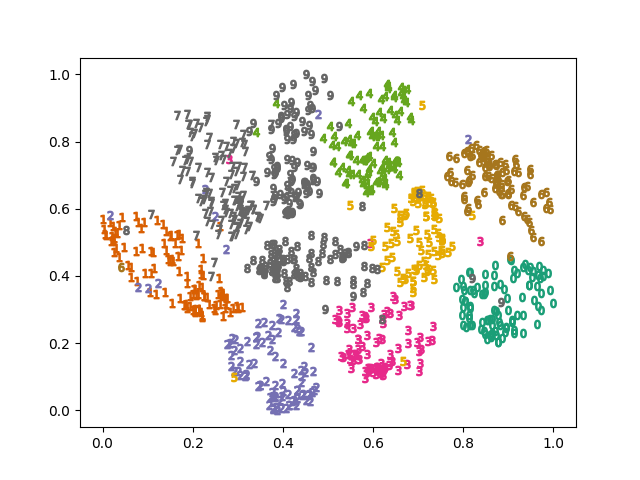
\includegraphics[width=.6\linewidth]{img/tsne_embedding.png}
    \caption{Wizualicacja docelowej przestrzeni t-SNE}\label{fig:tsne-embed}
\end{figure}

\pagebreak

\section{Wyniki eksperymentu --- Osoba 2 (Jakub Pawlak)}

Dla ekstrakcji cech w celu oceny separowalności wytrenowano sieć z małą ilością epok i oceniono macierz pomyłek, która znajduje się na rys~\ref{fig:hog-bad-cm}.

\begin{figure}[H]\centering
    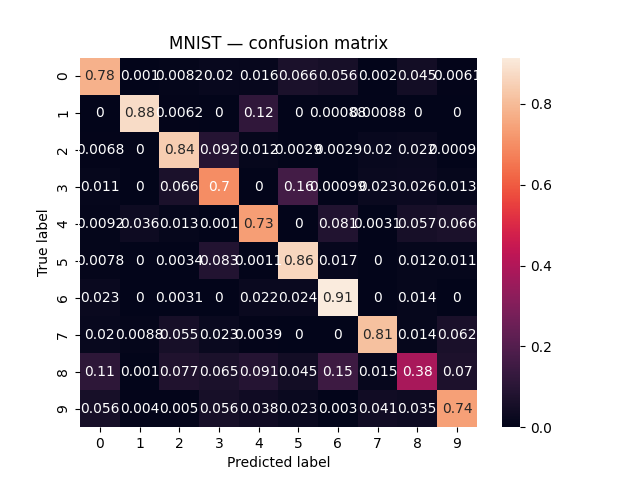
\includegraphics[width=.3\linewidth]{img/mnist_hog_bad_cm.png}
    \caption{Macierz pomyłek na słabo wytrenowanej sieci (ekstakcja HOG)}\label{fig:hog-bad-cm}
\end{figure}

Zauważyć można, że najgorzej model radzi sobie z rozpoznawaniem cyfr 8,3,4, 9 i 0.
Cyfra 8 bardzo często uznawana jest za 0,2,3,4 lub 6.
Często mylone są również 3 i 5.
Wynika to z faktu, że algorytm HOG wewnątrz komórek uzwględnia tylko ilość gradientów, a nie ich położenie względem siebie.
Dla przykładu, na rys.~\ref{fig:hig-similar} przedstawiono różne cyfry, które po ekstrakcji cech wyglądają podobnie.
Tak oto przedstawione cyfry 3 oraz 5 obie posiadają w prawej górnej ćwiartce linię ukośną i poziomą.
W cyfrze 3 linia pozioma idzie w prawo, a w cyfrze 5 --- w lewo, natomiast dla algorytmu HOG nie ma to znaczenia, ponieważ obie linie znajdują się w tej samej komórce.
Podobnie z cyframi 7 i 9, różniącymi się jedynie poziomym domknięciem, co jednak nie znajduje odzwierciedlenia w deskryprorze HOG, ponieważ pozioma linia już występuje gdzie indziej w tej samej ćwiartce.


\begin{figure}[H]\centering
    \begin{subfigure}[t]{.2\textwidth}
        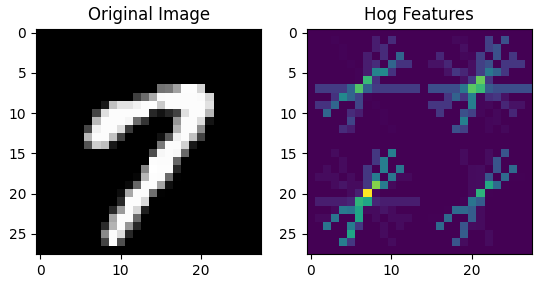
\includegraphics[width=\linewidth]{img/hog_similar/7.png}
        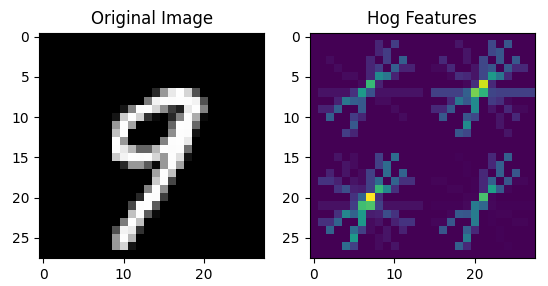
\includegraphics[width=\linewidth]{img/hog_similar/9.png}
        \caption{Podobne cechy dla różnych cyfr: 7 i 9}
    \end{subfigure}
    \hspace{.1\textwidth}
    \begin{subfigure}[t]{.2\textwidth}
        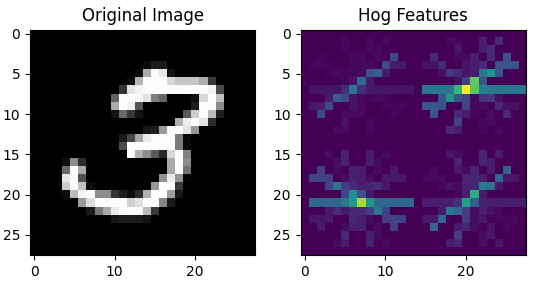
\includegraphics[width=\linewidth]{img/hog_similar/3.png}
        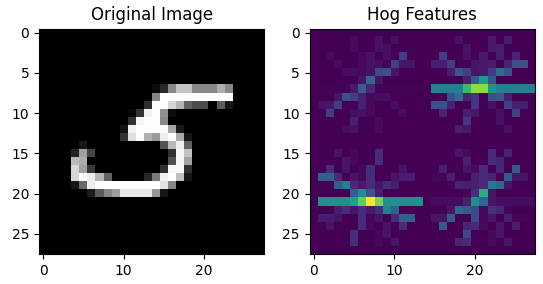
\includegraphics[width=\linewidth]{img/hog_similar/5.png}
        \caption{Podobne cechy dla różnych cyfr: 3 i 5}
    \end{subfigure}
    \caption{Różne cyfry, które posiadają podobne cechy}\label{fig:hig-similar}
\end{figure}

W metodzie t-SNE można ocenić separowalność wizualnie, na podstawie rys.~\ref{fig:tsne-embed},
jak również diagramu Woronoja na rys.~\ref{fig:tsne-voronoi}.
Od razu widać, że poszczególne klasy są separowalne, choć zdarzają się pola do pomyłek, zwłascze przy cyfrach 3,5 i 8, oraz 7,9 i 4.


\begin{figure}[H]\centering
    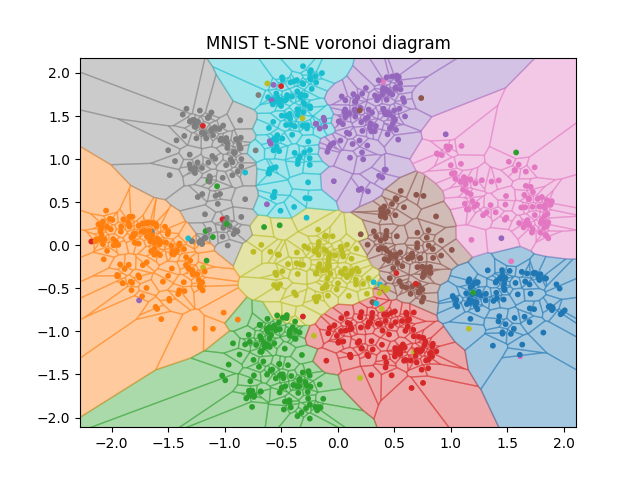
\includegraphics[width=.4\linewidth]{img/mnist_tsne_voronoi.png}
    \caption{Diagram Woronoja dla zbioru po przekształceniu t-SNE}\label{fig:tsne-voronoi}
\end{figure}


\pagebreak
\section{Wybór optymalnego modelu}

Podczas eksperymentów przeprowadzonych w ramach pierwszego projektu dało się zauważyć, że w miarę zwiększania
liczby neuronów w warstwie ukrytej, skuteczność ewentualnie ulegała wypłaszczeniu.
W takim przypadku, zwiększanie liczby neuronów skutkowałoby jedynie utrudnieniem obliczeń, bez pozytywnego efektu na skuteczności modelu.
Optymalnym modelem jest zatem taki, który maksymalizuje dokładność przy jednoczesnym minimalizowaniu ilości neuronów.

Przeprowadzone eksperymenty nie dostarczyły natomiast jednoznacznego sposobu, aby a priori określić najlepszą liczbę neuronów w warstwie ukrytej.
Wybór optymalnego modelu został dokonany poprzez coraz dokładnejsze przeszukiwanie przestrzeni liczb naturalnych, podobne w zasadzie działania do algorytmu \emph{binary search}.
Różne wartości liczby neuronów były poddawane procesowi uczenia, którego to wyniki pozwalały na oszacowanie, które wartości są najbardziej obiecujące.
Następnie wybierane zostały kolejne ilości neuronów do sprawdzenia --- tym razem z sąsiedztwa najlepiej spisujących się w poprzedniej iteracji.
Proces powtarzano, aż do znalezienia lokalnego maksimum skutecznośći.

Przykładowy przebieg pokazano na rys.~\ref{fig:hidden-size-choice}. Na wykresie pokazano zmianę wartości accuracy w zależności od rozmiaru warstwy ukrytej.
Najwyższe wartości udało się osiągnąć warstw ukrytych liczących 7 lub więcej neuronów. W takim przypadku zwiększenie liczby neuronów nie skutkuje poprawą skuteczności, więc preferowana jest wartość najmniejsza, t.j 7.

Metoda ta pozwoliła uzyskać satysfakcjonujące wyniki, jendak wskazać należy, że jesteśmy świadomi iż nie daje ona gwarancji, że wybrany model jest globalnie optymalny.

\begin{figure}[H]\centering
    \begin{tikzpicture}
        \begin{axis}[
                xlabel={rozmiar warstwy ukrytej},
                ylabel={accuracy [\%]}
            ]
            \addplot coordinates {
                    (2,93.33)
                    (3,96.67)
                    (4,96.67)
                    (5,96.67)
                    (6,90.00)
                    (7,100.00)
                    (8,100.00)
                    (9,100.00)
                    (10,100.00)
                };
        \end{axis}
    \end{tikzpicture}
    \caption{Przykładowe wartości accuracy dla różnych rozmiarów warstwy ukrytej na zbiorze Iris}\label{fig:hidden-size-choice}
\end{figure}

\pagebreak

\section{Wyniki klasyfikacji dla pierwszego sposobu ekstrakcji cech}

Poniżej przedtsawiono macierze pomyłek i wartości accuracy dla pozostałych zbiorów danych, oraz dla pierwzsej metody ekstrakcji cech ze zbioru MNIST.
Wszystkie sieci wykorzystują podobną architekturę, składającej się z warstwy wejściowej, jednej warstwy ukrytej i warstwy wyjściowej.
Rozmiar wartstw wejściowej i wyjściowej determinowany jest charakterystyką zbioru danych --- odpowiednio: ilością cech i ilością klas.
Rozmiar warstwy ukrytej został ustalony metodą opisaną na str.~5.
Wybrano możliwie małą wartość tak, aby jej zwiększenie nie powodowało poprawy skuteczności modelu.
Dodatkowo, w warstwie ukrytej aplikowana jest funkcja ReLU\@.

\begin{figure}[H]
    \centering
    \begin{subfigure}[t]{0.3\textwidth}
        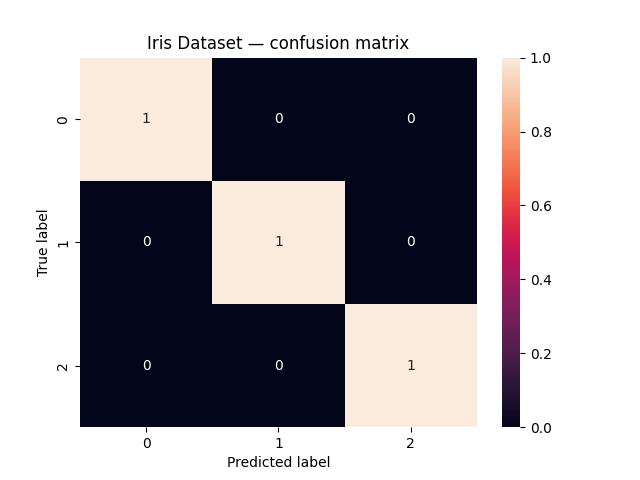
\includegraphics[width=\linewidth]{img/iris_cm.png}
        \caption{Zbior Iris}
    \end{subfigure}
    \hfill
    \begin{subfigure}[t]{0.3\textwidth}
        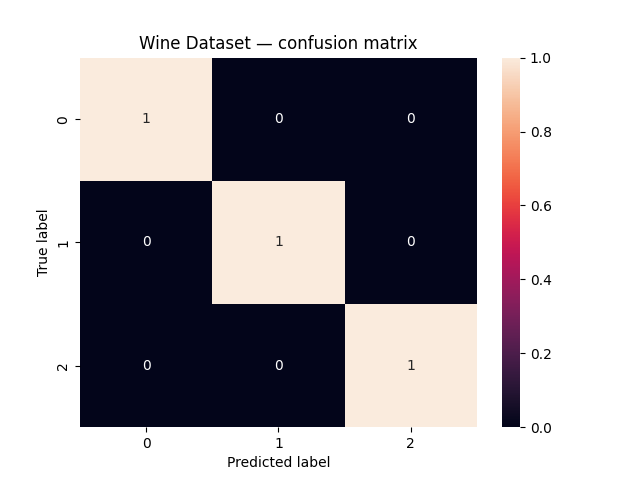
\includegraphics[width=\linewidth]{img/wine_cm.png}
        \caption{Zbior Wine}
    \end{subfigure}
    \hfill
    \begin{subfigure}[t]{0.3\textwidth}
        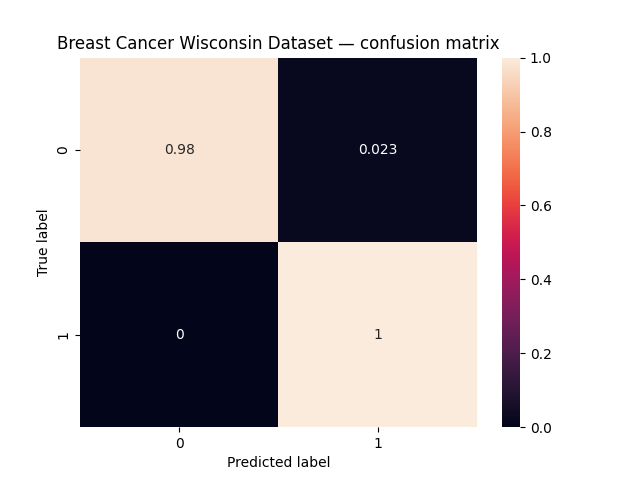
\includegraphics[width=\linewidth]{img/cancer_cm.png}
        \caption{Zbior Breast Cancer Wisconsin}
    \end{subfigure}
    \begin{subfigure}[t]{0.5\textwidth}
        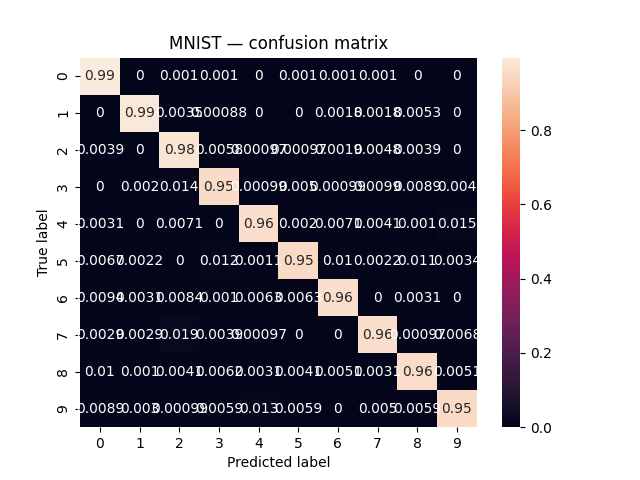
\includegraphics[width=\linewidth]{img/mnist_flat_cm.png}
        \caption{Zbior MNIST}
    \end{subfigure}
    \caption{Wyniki klasyfikacji dla 1 sposobu ekstrakcji cech}
\end{figure}

\begin{table}[H]\centering
    \begin{tabular}{lcc}
        \toprule
        Zbiór danych            & Wartość Accuracy & Rozmiar warstwy ukrytej \\
        \midrule
        Iris                    & 100\%            & 7                       \\
        Wine                    & 100\%            & 2                       \\
        Breast Cancer Wisconsin & 99.12\%          & 3                       \\
        MNIST                   & 97.16\%          & 64                      \\
        \bottomrule
    \end{tabular}
    \caption{Wartości accuracy wytrenowanego modelu}
\end{table}

Z wyników widać, że dla zbiorów Iris i Wine udało się uzyskać stuprocentową skuteczność.
Dziwne wydaje się, że dla zbioru Iris konieczne było użycie warstwy ukrytej większej od zarówno warstwy wejśćiowej jak i wyjściowej.
Dla zbioru Breast Cancer Wisconsin uzskano bardzo satysfakcjonujące 99.12\% accuracy.
Wynik 97\% dla zbioru mnist nie jest zadziwiający, biorąc pod uwagę, że niektóre cyfry są trudne do rozróżnienia nawet dla człowieka.
Nie jest zadziwiająca również najlepsza ilość neuronów w warstwie ukrytej, biorąc pod uwagę fakt, że warstwa wejściowa liczy ich 784.

\pagebreak

\section{Wyniki klasyfikacji --- Osoba 1 (Magdalena Pakuła)}
\pagebreak

\section{Wyniki klasyfikacji --- Osoba 2 (Jakub Pawlak)}

\subsection*{HOG}

Wyniki klasyfikacji z metodą HOG przedstawiono na rys.~\ref{fig:hog-cm}.
Widać znaczą poprawę w stosunku do wstępnych oczekiwań, choć tak jak przewidziano, z cyframi 2,3,7,8,9 model radzi sobie słabiej niż z resztą.
Tak jak przewidywano, często mylone są cyfry pary (2,3), (3,5), (7,9), (8,6), (8,9).
Ogólna wartość accuracy osiągnęła 89.21\%.

\begin{figure}[H]
    \centering
    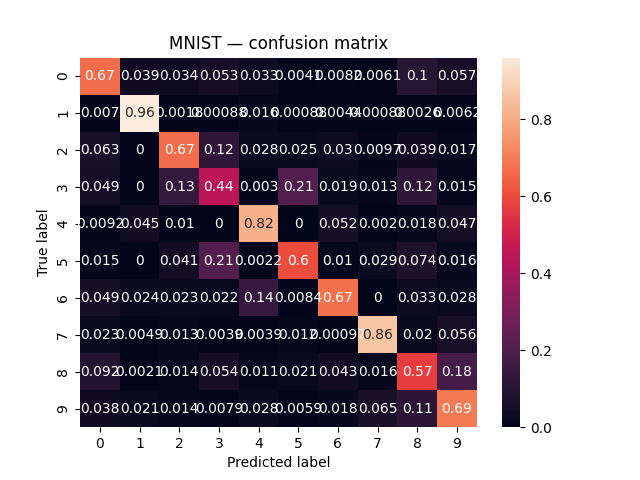
\includegraphics[width=.5\linewidth]{img/mnist_hog_cm.png}
    \caption{Wyniki klasyfikacji dla ekstrakcji cech metodą HOG (Accuracy: 89.21\%.)}\label{fig:hog-cm}
\end{figure}

\subsection*{t-SNE}

Na rys.~\ref{fig:tsne-cm} przestawiono macierz pomyłek oraz przebieg granicy decyzyjnej.
Model poradził sobie bardzo dobrze, jednak można zauważyć drobne pomyłki.
Zgodnie z przewidywaniami, 4 i 7 były często uznawane za 9, jak również mylone były cyfry z grupy 3,5,8.
Pomimo mniejszej liczby cech, model osiągnął lepszą niż w poprzedniej metodzie wartość accuracy wynoszącą 95.67\%.
Wskazać jednak należy istotną wadę tej metody, mianowicie t-SNE operuje na całym zbiorze danych, więc użycie tej metody
ekstrakcji cech nie będzie można zastosować w przypadku pojawnienia się nowych danych.

\begin{figure}[H]
    \centering
    \begin{subfigure}[t]{.5\textwidth}\centering
        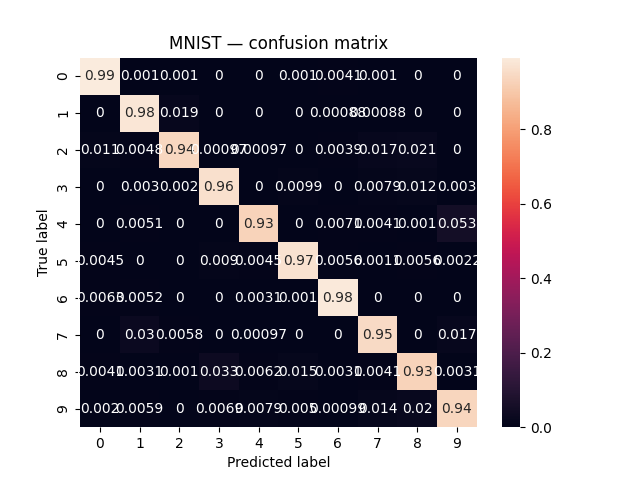
\includegraphics[width=\linewidth]{img/mnist_tsne_cm.png}
        \caption{Macierz pomyłek}\label{fig:tsne-cm}
    \end{subfigure}
    \hspace{-3em}
    \begin{subfigure}[t]{.5\textwidth}\centering
        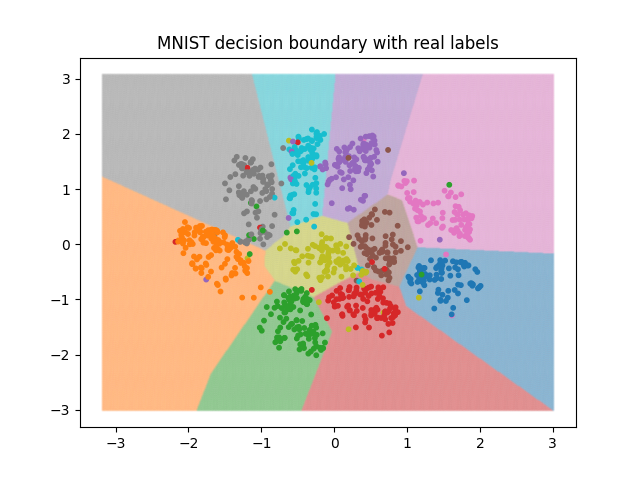
\includegraphics[width=\linewidth]{img/mnist_tsne_db.png}
        \caption{Granice decyzyjne}\label{fig:tsne-db}
    \end{subfigure}
    \caption{Wyniki klasyfikacji dla ekstrakcji cech metodą t-SNE (Accuracy: 95.67\%)}
\end{figure}

Z obydwu eksperymentów dojść można do wniosku, 
że ręczna ekstrakcja cech nie jest zadaniem łatwym, 
ponieważ w obu przypadkach poskutkowała ona pogorszeniem skuteczności modelu.





\end{document}